\documentclass[10pt]{article}
\usepackage[T1]{fontenc}
\usepackage{lmodern,amsmath,amssymb,graphicx,hyperref,array}
\usepackage[margin=.78in]{geometry}
\setlength{\parindent}{0pt}\setlength{\parskip}{6pt}
\begin{document}
\begin{center}{\Large The actual norm has a canonical quadratic residual}\\[3pt]
23 November 2026 --- fixed-support local unsigned Lean evidence\end{center}
\textbf{Exact setting.}
Let $K$ be a field, $2\ne0$, $\deg f=3$.
Let $S$ have three elements with an explicit
$e:\operatorname{Fin}(3)\simeq S$; require $x_t\notin S$,
nonzero $y_t,z(x)$, and actual point equations
$y_t^2=f(x_t)$, $z(x)^2=f(x)$ for $x\in S$.
The actual original interpolation operator has72coefficient coordinates
and70mixed-jet rows. There is a vector $v$ in its kernel whose actual
curve remainder is $A+BY$ and whose actual norm $N=A^2-fB^2$ satisfies
\[
 N\ne0,\quad \deg N\le30,\qquad
 L=(X-x_t)^4\prod_{x\in S}(X-x)^8,
\]
\[
 Q=N/_{\!m}L,\qquad N=LQ,\quad Q\ne0,\quad\deg Q\le2.
\]
The forced factor $L$ is actually monic of exact degree28.
The quotient is constructed by division by that monic polynomial;
$Q$ itself is not claimed monic. No successful factor or quotient witness
is supplied (PCC-20261123-148f8a,6e7e87) [pcc:unverified].

\begin{center}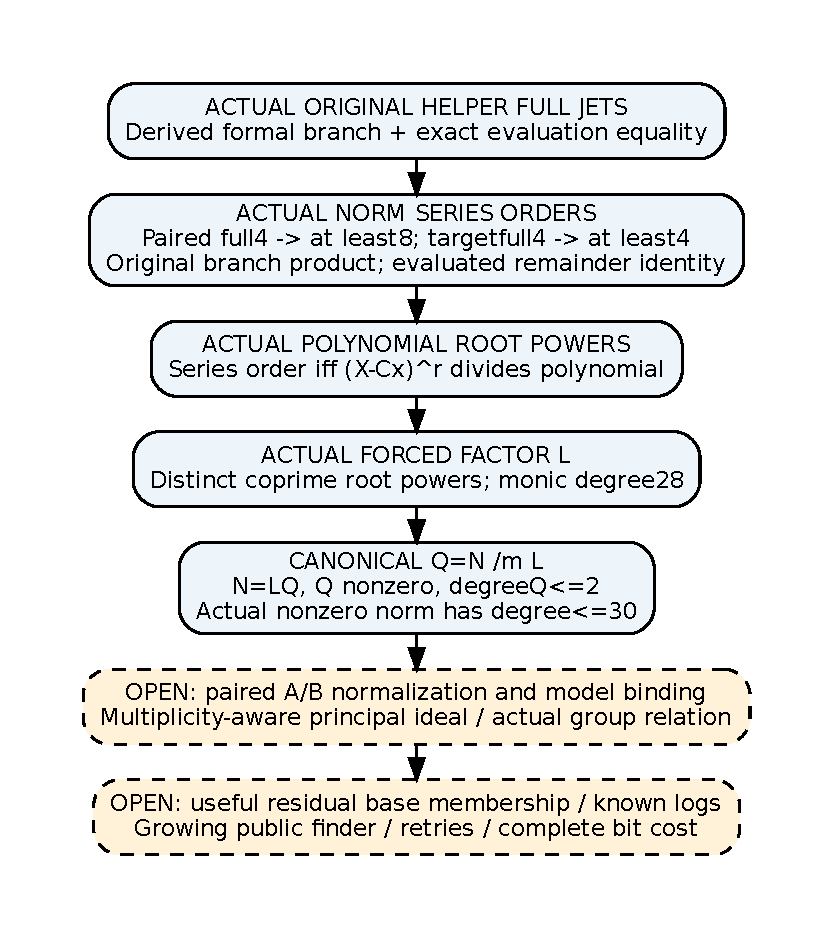
\includegraphics[width=.87\linewidth,height=.52\textheight,keepaspectratio]{norm-factors-dependencies-001.pdf}\end{center}
\textbf{What is checked.}
Source056/build059/local029 accepts147primary statements,14new since133,
exit zero, no warnings, all printed dependencies standard.
The result is local unsigned data, outside shared Transport53/57
audit/fresh. Fixed support four is explicit; no growing algorithm,
residual splitting or scalar labels follow from the degree bound
[pcc:unverified].
\newpage
\begin{center}{\Large From original jets to the actual polynomial factors}\end{center}
\textbf{1. Derive the branch and original evaluation.}
At an actual point, $g=f(Cx+T)$ has constant coefficient $y^2$.
The existing complete-ring Hensel theorem supplies
$s=Cy+Tu$ with $s^2=g$, using the actual unit $2y$.
The generic exact two-Taylor/swap identity now identifies the explicit
translated evaluation with the original helper at $(Cx+T,Cy+Tu)$.
The study's actual full mixed multiplicity $r$ therefore gives
$T^r$ divisibility of the original branch evaluation.
No desired evaluation equality or successful branch is assumed
[pcc:unverified].

\textbf{2. Reduce at the root, not in ambient jet space.}
Existing monic-division evaluation at a root gives equality between
evaluated original helper and its actual curve remainder.
Consequently the actual norm evaluated at $Cx+T$ is exactly
the product of original helper evaluations at $s$ and $-s$.
Paired full multiplicity $r$ gives norm order at least $2r$.
A singleton branch gives at least $r$, with no extra order assumed.
There is no assertion that ambient jets of the remainder are preserved
(PCC-20261123-148f8a) [pcc:unverified].

\textbf{3. Convert order to factors.}
A separate generic owner theorem proves, over any commutative ring,
\[
 T^r\mid p(Cx+T)\ \Longleftrightarrow\ (X-Cx)^r\mid p.
\]
It uses actual polynomial-to-series coefficients and Taylor translation
in both directions, including zero and $r=0$ cases.
Apply it to the actual norm series orders, obtaining target power four
and each paired power eight. Actual distinct abscissas make these
polynomial factors coprime, so their product divides $N$
(PCC-20261123-6e7e87) [pcc:unverified].

\textbf{4. Construct and bound the quotient.}
The monic factor product has degree $4+3\cdot8=28$.
Actual division gives $N=LQ$; $N\ne0$ forces $Q\ne0$.
Exact product degree and the derived norm cap yield
$28+\deg Q=\deg N\le30$. Thus $\deg Q\le2$; no quotient degree premise
is supplied [pcc:unverified].

\textbf{Proof map and standing.}
Namespace \texttt{OrientationActualNormSeries} contains seven endpoints
for original substitution order, branch/order existence, evaluated
remainder, norm product, paired/single order and actual norm witness
(source055/build058/local028,140total).
Namespace \texttt{OrientationActualNormFactors} contains seven endpoints
for monicity, degree, divisibility, canonical reconstruction, nonzero
quotient, degree and actual witness
(source056/build059/local029,147total) [pcc:unverified].

Generic owner \texttt{PolynomialMixedEvaluation} has four separately
built/audited statements at commit \texttt{653983f}.
\texttt{PolynomialSeriesRootOrder} has three at
\texttt{04d23b3}. Each focused build exits zero without warnings;
unchanged audits report zero failing/extra trusted.
PCC cf5d6c/1ab62b and8d6473/7df68a have prefixPCC-20261123- and remain
unsigned. Lean4.35.0 and exact Mathlib/input bytes are pinned.
Local60/65-file compiled overlays preserve old modules without manifest,
umbrella, gate, trust or CI changes; no whole-project/fresh standing
is inferred [pcc:unverified].
\newpage
\begin{center}{\Large The scalar-recovery test remains separate}\end{center}
\textbf{Prior group work exists and has precise hypotheses.}
The source review of \texttt{NormGroupBridge} records:
\begin{itemize}
\item \texttt{principalPointProduct}: actual nonsingular points with
injective abscissas, a nonzero coordinate-ring function in their
point ideals, and norm degree equal to the number of those points.
\item \texttt{fullNormPointSum}: short-form coefficients and a norm
equal to a nonzero constant times a nodal polynomial on distinct points.
\item \texttt{targetScalarFromSum}: an actual point sum plus supplied
integer labels for every other point.
\end{itemize}
These earlier results are not newly audited or absent. Their simple-point,
nodal-norm and supplied-label premises are not automatic for the current
repeated factors. Source-only reviewPCC-20261123-8fa3bdpins the exact
statements and prior report [pcc:unverified].

Current algebra requires a cubic and local nonzero ordinates; it does
not already bind a globally nonsingular elliptic group or prime subgroup.
A group theorem must specialize $f$ to the actual Weierstrass cubic,
match the $A+BY$ convention to the prior $A-BY$ function, retain
nonsingularity, and account for all multiplicities and exceptional cases.

\textbf{Next discriminating construction.}
For actual $G=\prod_{x\in S}(X-x)$, test
\[
 G^4\mid A,\ B;\qquad
 A=G^4A',\ B=G^4B',\quad
 \deg A'\le3,\ \deg B'\le1.
\]
This normalization is prospective, not part of147.
Use both actual remainder branch evaluations: their difference contains
$2sB$. The actual constant coefficient and $2y\ne0$ make $2s$ a unit,
so series divisibility could be cancelled; then recover $A$ by subtraction
and convert to actual polynomial factors.
Canonical division must produce $A',B'$ and their bounds.
This tests which group information the paired support contributes
[pcc:unverified].

Only after that construction should the function be mapped to actual
principal point ideals and the elliptic point group. Repeated target
multiplicity, residual degree zero/one/two, base-field splitting,
infinity, zero denominators and duplicate/ramified cases must be
handled explicitly. A successful quadratic root extraction does not
itself give those points' discrete logarithms or useful known-log
factor-base membership.

\textbf{Original acceptance criteria are unchanged.}
The goal concerns public inputs on general nonsingular $E/\mathbb F_p$,
$p>3$, with a prime-order subgroup and $\log p=O(\log r)$.
There is no weak-curve or reusable-precomputation shortcut.
An actual public finder, field/scalar correctness, coverage/retries and
complete expected $\exp(o(\log r))$ bit cost remain open.
The original nonscalar-origin and rank-directed $W$-jet mechanisms
remain separate unbound proposals. The fixed four-point factor result
does not establish an algorithm or universal nonexistence.

\textbf{Preservation.}
All prior sources, raw logs, claims, local ledger prefix and immutable
pending/final reports remain exact. No mathematical candidate failed
in these two new consumer stages; one generic report layout revision
is retained. Existing branch-selection problem has a dated prefix
append and index update with its original exit criteria.
Protected canonical ledger divergence still blocks remote publication;
no push/rechain/reissue/signing/gate bypass, watcher edit,
paid/cloud/native/attack or timing/scaling campaign was used.
\end{document}
